\chapter{Rotational and Vibrational Spectroscopy}\label{ch:b3:rovibrational-spectroscopy}

On a high, dry plateau, dozens of radio antennas point at a dark cloud
between the stars. Among the frequencies they collect is one at
\qty{115.271}{GHz}: carbon monoxide molecules, at a few kelvin, turning
from their first rotational level to the lowest. From that single number a
chemist obtains the length of the C--O bond to a fraction of a picometre; from
the strengths of the next lines, the temperature of the cloud. The
rotations and vibrations of molecules are the subject of this chapter: their
levels, from the rotor and the oscillator of
\cref{ch:b3:quantum-model-systems}; the selection rules, from
\cref{ch:b3:group-theory-applied}; and what spectra measure --- bond
lengths, \omterm{def:b3:quantum-model-systems:oscillator}{force constants}, dissociation energies.

\begin{recall}
\Cref{ch:b3:quantum-model-systems} gave the \omterm{def:b3:quantum-model-systems:rotor}{rigid rotor}, $E_J = J(J+1)\hbar^2/2I$
with \omterm{def:b3:quantum-model-systems:degenerate}{degeneracy} $2J + 1$, and the \omterm{def:b3:quantum-model-systems:oscillator}{harmonic oscillator}, $E_v = (v + \frac12)h\nu$,
for a diatomic of \omterm{def:b3:quantum-model-systems:oscillator}{reduced mass} $\mu$. \Cref{ch:b3:group-theory-applied} stated
the infrared and Raman selection rules. The Year 1 volume measured infrared
spectra in wavenumbers and defined the polarisability of a molecule.
\end{recall}

\begin{omfigure}
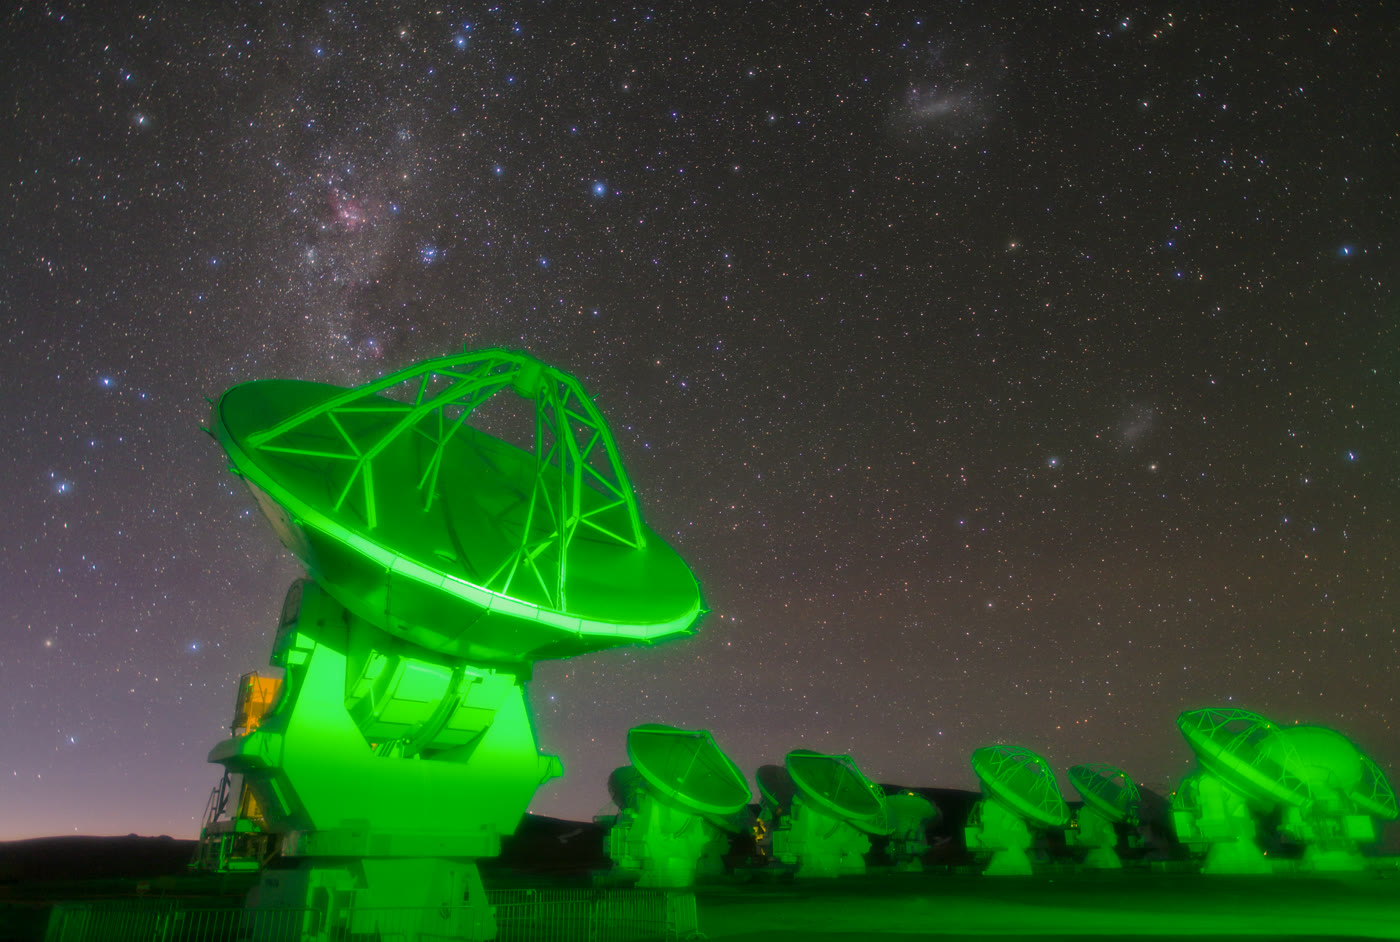
\includegraphics[width=0.7\linewidth]{images/book4/alma-antennas.jpg}

{\small Antennas of a radio interferometer on a high plateau: they record,
among many others, the rotational lines of carbon monoxide from interstellar
clouds. Photograph ESO/B.~Tafreshi (twanight.org), CC BY 4.0.}
\end{omfigure}

\section{Rotational spectra}

\begin{definition}[Rotational constant, isotopologue]\label{def:b3:rovibrational-spectroscopy:rotational-constant}
The \emph{rotational constant}\index{rotational constant} of a linear molecule
is $B = h/(8\pi^2cI)$, in \unit{cm^{-1}} (or $B = h/8\pi^2I$ in hertz), so that its
rotational levels are $F(J) = BJ(J+1)$ in wavenumbers. Molecules that differ
only in the isotopes of their atoms are \emph{isotopologues}\index{isotopologue}
(\ce{^{12}C^{16}O}, \ce{^{13}C^{16}O}); in the \omterm{def:b3:computational-chemistry:born-oppenheimer}{Born--Oppenheimer approximation}
they share the same bond lengths and \omterm{def:b3:quantum-model-systems:oscillator}{force constants}.
\end{definition}

\begin{definition}[Gross and specific selection rules]\label{def:b3:rovibrational-spectroscopy:selection}
A \emph{gross selection rule}\index{gross selection rule} states which
property a molecule must have to show a kind of spectrum at all; a
\emph{specific selection rule}\index{specific selection rule} states which
changes of quantum number are allowed.
\end{definition}

\begin{proposition}[Pure rotational spectra]\label{prop:b3:rovibrational-spectroscopy:rotational-lines}
A molecule has a pure rotational (microwave) spectrum only if it has a
permanent dipole moment; for a linear molecule the specific rule is $\Delta J
= \pm1$. Absorption lines lie at
\[
\tilde\nu = F(J+1) - F(J) = 2B(J + 1), \qquad J = 0, 1, 2, \dots,
\]
equally spaced by $2B$.
\end{proposition}

\begin{proof}
The interaction with light is through the dipole moment: a molecule with no
permanent dipole has no oscillating dipole when it rotates. The rule $\Delta J
= \pm1$ comes from the vanishing of $\int Y_{J'M'}^*\cos\theta\,Y_{JM}$ unless $J' = J
\pm 1$ (the dipole component along $z$ transforms like $Y_{1,0}$), admitted.
Then $B(J+1)(J+2) - BJ(J+1) = 2B(J+1)$.
\end{proof}

\begin{method}[Bond length from a rotational line]\label{met:b3:rovibrational-spectroscopy:bond-length}
\begin{enumerate}
  \item From the line $J + 1 \leftarrow J$ at frequency $\nu$, deduce $B =
        \nu/2(J+1)$ (in hertz).
  \item Compute the moment of inertia $I = h/8\pi^2B$.
  \item With the \omterm{def:b3:quantum-model-systems:oscillator}{reduced mass} from isotopic masses, $r = \sqrt{I/\mu}$.
\end{enumerate}
\end{method}

\begin{example}[Carbon monoxide]\label{ex:b3:rovibrational-spectroscopy:co}
% ledger: rotl:CO.1-0, imass:O16
The line $J = 1 \leftarrow 0$ of \ce{^{12}C^{16}O} is at \qty{115271.20}{MHz}:
$B = \qty{57635.6}{MHz} = \qty{1.92252}{cm^{-1}}$, $I = \qty{1.4560e-46}{kg.m^2}$.
With $\mu = 12 \times 15.99491/27.99491 = \qty{6.85621}{u}$, $r_0 = \qty{113.09}{pm}$.
This $r_0$ averages the bond over its zero-point vibration and is slightly
longer than the equilibrium length $r_e$ (\cref{sec:b3:rovibrational-spectroscopy:real-bonds}).
\end{example}

\begin{definition}[Centrifugal distortion constant]\label{def:b3:rovibrational-spectroscopy:centrifugal}
A rotating bond stretches; the levels become $F(J) = BJ(J+1) - DJ^2(J+1)^2$,
where $D$ is the \emph{centrifugal distortion constant}\index{centrifugal distortion constant},
and the lines $2B(J+1) - 4D(J+1)^3$ close up slowly at
high $J$.
\end{definition}

\begin{proposition}[The strongest line]\label{prop:b3:rovibrational-spectroscopy:jmax}
If line intensities follow the population of the lower level, $(2J+1)
\eu^{-hcBJ(J+1)/kT}$, the most populated level is near
\[
J_{\max} \approx \sqrt{\frac{kT}{2hcB}} - \frac12.
\]
\end{proposition}

\begin{proof}
Treat $J$ as continuous and differentiate: $\frac{\dd}{\dd J}[(2J+1)\eu^{-aJ(J+1)}]
= [2 - a(2J+1)^2]\eu^{-aJ(J+1)}$ with $a = hcB/kT$; it vanishes at $(2J + 1)^2 =
2/a$.
\end{proof}

\begin{omfigure}
\begin{tikzpicture}
\begin{axis}[width=0.9\linewidth, height=4.8cm, xmin=0, xmax=70, ymin=0,
  ymax=1.12, ytick=\empty, axis x line=bottom, axis y line=left, ycomb,
  xlabel={wavenumber / cm$^{-1}$}, ylabel={relative intensity},
  tick label style={font=\small}, label style={font=\small}]
\addplot[omDef, very thick] table[x=nu, y=I] {figdata/out/bachelor-3-rotational-spectrum-co-30.dat};
\addplot[omThm, thick, xshift=1.2pt] table[x=nu, y=I] {figdata/out/bachelor-3-rotational-spectrum-co-300.dat};
\end{axis}
\end{tikzpicture}

{\small The rotational absorption spectrum of carbon monoxide, lines spaced
by $2B = \qty{3.845}{cm^{-1}}$, intensities taken as the population of the
lower level, at \qty{30}{K} (blue) and \qty{300}{K} (red, shifted slightly for
visibility), each temperature scaled to its strongest line. At \qty{30}{K} the strongest line is
$J = 3 \leftarrow 2$; at \qty{300}{K}, $J = 8 \leftarrow 7$.}
\end{omfigure}

\section{Vibrations of real bonds}\label{sec:b3:rovibrational-spectroscopy:real-bonds}

A real bond does not obey Hooke's law far from equilibrium: it softens when
stretched and breaks.

\begin{definition}[Morse potential]\label{def:b3:rovibrational-spectroscopy:morse}
The \emph{Morse potential}\index{Morse potential} is $V(r) = D_e[1 -
\eu^{-\beta(r - r_e)}]^2$: harmonic near $r_e$ (\omterm{def:b3:quantum-model-systems:oscillator}{force constant} $2\beta^2D_e$), and
tending to the dissociation limit $D_e$ at large $r$.
\end{definition}

\begin{proposition}[Levels of the Morse oscillator]\label{prop:b3:rovibrational-spectroscopy:morse-levels}
In wavenumbers the vibrational levels of a Morse oscillator are
\[
G(v) = \tilde\omega_e(v + \tfrac12) - \tilde\omega_ex_e(v + \tfrac12)^2, \qquad
\tilde\omega_ex_e = \frac{\tilde\omega_e^2}{4D_e},
\]
a ladder whose rungs close up and end at $v_{\max} = \lfloor\tilde\omega_e/
2\tilde\omega_ex_e - \frac12\rfloor$.
\end{proposition}
\admitted

The solution of the Morse equation is treated in more advanced courses;
the levels are checked numerically in this chapter's figure data.

\begin{definition}[Anharmonicity constant, fundamental, overtone, hot band]\label{def:b3:rovibrational-spectroscopy:anharmonic}
$\tilde\omega_ex_e$ is the \emph{anharmonicity constant}\index{anharmonicity constant}.
The \emph{fundamental transition}\index{fundamental transition}
is $v = 1 \leftarrow 0$; an \emph{overtone}\index{overtone} is $v = n \leftarrow 0$
with $n \ge 2$, weak because the gross rule $\Delta v = \pm1$ of the \omterm{def:b3:quantum-model-systems:oscillator}{harmonic
oscillator} is only slightly broken; a \emph{hot band}\index{hot band} starts
from an excited level, $v = 2 \leftarrow 1$, and grows with temperature.
\end{definition}

\begin{definition}[Spectroscopic dissociation energy]\label{def:b3:rovibrational-spectroscopy:dissociation}
The \emph{spectroscopic dissociation energy}\index{spectroscopic dissociation energy}
of a molecule is the depth of its potential, $D_e$, measured from the
minimum, or $D_0 = D_e - G(0)$, measured from the lowest level --- per
molecule at \qty{0}{K}, unlike the bond dissociation enthalpy of the Year 2
volume, a molar enthalpy at \qty{298}{K}.
\end{definition}

\begin{corollary}[$D_e$ and $D_0$ of a Morse oscillator]\label{cor:b3:rovibrational-spectroscopy:de}
$D_e = \tilde\omega_e^2/4\tilde\omega_ex_e$ and $D_0 = D_e - (\frac12\tilde\omega_e -
\frac14\tilde\omega_ex_e)$.
\end{corollary}

\begin{proof}
The first is the relation of the proposition; the second is $G(0)$.
\end{proof}

\begin{proposition}[Birge--Sponer extrapolation]\label{prop:b3:rovibrational-spectroscopy:birge-sponer}
The gaps $\Delta G(v + \frac12) = G(v+1) - G(v) = \tilde\omega_e - 2\tilde\omega_ex_e(v +
1)$ decrease linearly with $v$; summing them until they vanish gives $D_0$, the
area under the plot of $\Delta G$ against $v$.
\end{proposition}

\begin{proof}
Subtract the two expressions of $G$. $D_0$ is the energy from $v = 0$ to the
limit, the sum of all the gaps.
\end{proof}

\begin{example}[Hydrogen chloride]\label{ex:b3:rovibrational-spectroscopy:hcl}
% ledger: diat:HCl.we, diat:HCl.wexe, janaf:H.dfH0, janaf:Cl.dfH0, janaf:HCl.dfH0
For \ce{H^{35}Cl}, $\tilde\omega_e = \qty{2990.95}{cm^{-1}}$ and $\tilde\omega_ex_e =
\qty{52.82}{cm^{-1}}$: the fundamental is at $\tilde\omega_e - 2\tilde\omega_ex_e =
\qty{2885.3}{cm^{-1}}$ and the first \omterm{def:b3:rovibrational-spectroscopy:anharmonic}{overtone} at $2\tilde\omega_e - 6\tilde\omega_ex_e =
\qty{5665.0}{cm^{-1}}$, slightly less than twice the fundamental. The Morse model
predicts $D_e = \qty{42342}{cm^{-1}}$ and $D_0 = \qty{40860}{cm^{-1}}$; the true $D_0$,
from the enthalpies of formation of H, Cl and HCl at \qty{0}{K}, is
\qty{35760}{cm^{-1}} (\qty{4.43}{eV}). The real potential flattens out faster than a
Morse curve fitted at the bottom: Birge--Sponer extrapolations from the
lowest levels overestimate dissociation energies.
\end{example}

\begin{omfigure}
\begin{tikzpicture}
\begin{axis}[name=morse, width=0.55\linewidth, height=6cm, xmin=0.8, xmax=4.0,
  ymin=0, ymax=48000, axis lines=left, xlabel={$r$ / \AA}, ylabel={$V$ / cm$^{-1}$},
  unbounded coords=jump, scaled y ticks=false, ytick={0,10000,20000,30000,40000},
  tick label style={font=\small}, label style={font=\small}]
\addplot[black, thick] table[x=r, y=V] {figdata/out/bachelor-3-morse-levels.dat};
\addplot[gray, dashed] table[x=r, y=harm] {figdata/out/bachelor-3-morse-levels.dat};
\addplot[omDef] table[x=r, y=E] {figdata/out/bachelor-3-morse-levels-levels.dat};
\draw[<->, omThm] (axis cs:3.7,0) -- (axis cs:3.7,42342) node[pos=0.5, left, font=\small] {$D_e$};
\draw[dashed, omThm] (axis cs:1.2,42342) -- (axis cs:4.0,42342);
\end{axis}
\begin{axis}[at={(morse.east)}, anchor=west, xshift=1.6cm, width=0.4\linewidth,
  height=5cm, xmin=0, xmax=28, ymin=0, ymax=3100, axis lines=left,
  xlabel={$v$}, ylabel={$\Delta G(v + \frac12)$ / cm$^{-1}$},
  tick label style={font=\small}, label style={font=\small}]
\addplot[omDef, only marks, mark size=1.2pt] table[x=v, y=dG] {figdata/out/bachelor-3-morse-levels-bs.dat};
\addplot[omDef!40, fill=omDef!12, draw=none] table[x=v, y=dG] {figdata/out/bachelor-3-morse-levels-bs.dat} \closedcycle;
\end{axis}
\end{tikzpicture}

{\small Left: the \omterm{def:b3:rovibrational-spectroscopy:morse}{Morse potential} of \ce{HCl} built from its spectroscopic
constants (solid), the harmonic parabola with the same curvature (dashed),
and every third vibrational level, drawn between its turning points; the
levels close up towards $D_e$. Right: the Birge--Sponer plot of the gaps;
the shaded area is $D_0$.}
\end{omfigure}

\section{Rovibrational bands}

A vibrational transition of a gas is accompanied by rotational changes, $\Delta
J = \pm1$ for a diatomic in a ${}^1\Sigma$ state.

\begin{definition}[P, Q and R branches, band origin]\label{def:b3:rovibrational-spectroscopy:branches}
In a rovibrational band, the lines with $\Delta J = -1$ form the \emph{P
branch}\index{P branch}, those with $\Delta J = +1$ the \emph{R branch}\index{R branch},
and those with $\Delta J = 0$, when allowed, the \emph{Q branch}\index{Q branch}.
The \emph{band origin}\index{band origin} $\tilde\nu_0$ is the
vibrational energy difference without rotation.
\end{definition}

\begin{theorem}[Combination differences]\label{thm:b3:rovibrational-spectroscopy:combination-differences}
With \omterm{def:b3:rovibrational-spectroscopy:rotational-constant}{rotational constants} $B_0$ and $B_1$ in the lower and upper vibrational
levels, $R(J) = \tilde\nu_0 + B_1(J+1)(J+2) - B_0J(J+1)$ and $P(J) = \tilde\nu_0 +
B_1(J-1)J - B_0J(J+1)$, and
\[
R(J - 1) - P(J + 1) = 4B_0(J + \tfrac12), \qquad R(J) - P(J) = 4B_1(J + \tfrac12).
\]
\end{theorem}

\begin{proof}
The first two follow from $E = G(v) + B_vJ(J+1)$ for both levels. $R(J - 1)$ and
$P(J + 1)$ end on the same upper level $J$, from lower levels $J - 1$ and $J + 1$:
their difference is $B_0[(J+1)(J+2) - (J-1)J] = B_0(4J + 2)$. Likewise $R(J)$ and
$P(J)$ start from the same lower level and end on $J + 1$ and $J - 1$.
\end{proof}

\begin{method}[Analysing a rovibrational band]\label{met:b3:rovibrational-spectroscopy:combination}
\begin{enumerate}
  \item Locate the gap: for a ${}^1\Sigma$ diatomic there is no \omterm{def:b3:rovibrational-spectroscopy:branches}{Q branch}, and
        $\tilde\nu_0$ lies in the gap, between $R(0)$ and $P(1)$.
  \item Number the lines outwards from the gap: $R(0), R(1), \dots$ and $P(1),
        P(2), \dots$.
  \item Use the combination differences to get $B_0$ and $B_1$
        separately, then $\alpha_e = B_0 - B_1$ and $B_e = B_0 + \frac12\alpha_e$.
\end{enumerate}
\end{method}

\begin{omfigure}
\begin{tikzpicture}
\begin{axis}[width=0.92\linewidth, height=5cm, xmin=2650, xmax=3080, ymin=0,
  ymax=1.15, ytick=\empty, axis x line=bottom, axis y line=left,
  xlabel={wavenumber / cm$^{-1}$}, ylabel={absorbance (relative)},
  tick label style={font=\small}, label style={font=\small}]
\addplot[omDef, thin] table[x=nu, y=A] {figdata/out/bachelor-3-rovib-band.dat};
\node[font=\small] at (axis cs:2780,1.06) {P branch};
\node[font=\small] at (axis cs:2985,1.06) {R branch};
\draw[->, gray] (axis cs:2885.3,0.45) -- (axis cs:2885.3,0.05);
\node[font=\small, gray, anchor=south] at (axis cs:2885.3,0.45) {$\tilde\nu_0$};
\end{axis}
\end{tikzpicture}

{\small The fundamental band of gaseous \ce{HCl} at \qty{300}{K}, computed from
its spectroscopic constants: P and \omterm{def:b3:rovibrational-spectroscopy:branches}{R branches} either side of the gap at the
\omterm{def:b3:rovibrational-spectroscopy:branches}{band origin}. Each line is a doublet, \ce{H^{35}Cl} and the weaker, slightly
lower \ce{H^{37}Cl} (natural abundances 76\,\% and 24\,\%). The R lines close up,
the P lines spread out, because $B_1 < B_0$.}
\end{omfigure}

\begin{example}[The constants of \ce{HCl} from its band]\label{ex:b3:rovibrational-spectroscopy:analysis}
% ledger: diat:HCl.Be, diat:HCl.ae
With $R(0) = \qty{2905.58}{cm^{-1}}$ and $P(2) = \qty{2842.94}{cm^{-1}}$, one finds
$6B_0 = \qty{62.64}{cm^{-1}}$, so $B_0 = \qty{10.440}{cm^{-1}}$. With $R(1) = 2925.23$ and $P(1) =
\qty{2864.43}{cm^{-1}}$, $B_1 = \qty{10.133}{cm^{-1}}$. So $\alpha_e = \qty{0.307}{cm^{-1}}$
and $B_e = \qty{10.593}{cm^{-1}}$, the values the band was built from:
the method recovers them exactly.
\end{example}

\section{Raman spectroscopy}

\begin{definition}[Raman and Rayleigh scattering]\label{def:b3:rovibrational-spectroscopy:raman}
When light of frequency $\nu_0$ crosses a sample, most of the scattered light
keeps the frequency $\nu_0$: \emph{Rayleigh scattering}\index{Rayleigh scattering}.
A small fraction is shifted by the rotational or vibrational
frequencies of the molecules: \emph{Raman scattering}\index{Raman scattering}.
Lines at lower frequency are \emph{Stokes lines}\index{Stokes line} (the
molecule gained energy), at higher frequency \emph{anti-Stokes
lines}\index{anti-Stokes line} (it lost energy).
\end{definition}

\begin{proposition}[Classical origin of the Raman effect]\label{prop:b3:rovibrational-spectroscopy:raman-classical}
If the polarisability of a molecule vibrating at $\nu_{\mathrm{vib}}$ varies
as $\alpha = \alpha_0 + \alpha_1\cos(2\pi\nu_{\mathrm{vib}}t)$, the dipole induced by a
field $E_0\cos(2\pi\nu_0t)$ oscillates at $\nu_0$ and at $\nu_0 \pm \nu_{\mathrm{vib}}$.
A vibration is \omterm{def:b3:group-theory-applied:activity}{Raman active} only if it changes the polarisability.
\end{proposition}

\begin{proof}
$\mu = \alpha E = \alpha_0E_0\cos(2\pi\nu_0t) + \frac12\alpha_1E_0[\cos2\pi(\nu_0 +
\nu_{\mathrm{vib}})t + \cos2\pi(\nu_0 - \nu_{\mathrm{vib}})t]$, by $\cos a\cos b =
\frac12[\cos(a+b) + \cos(a-b)]$. Each oscillating dipole radiates at its own
frequency; without $\alpha_1$ only the Rayleigh term remains.
\end{proof}

\begin{proposition}[Rotational Raman lines]\label{prop:b3:rovibrational-spectroscopy:rotational-raman}
A linear molecule with an anisotropic polarisability shows rotational Raman
lines with $\Delta J = \pm2$, displaced from the exciting line by
\[
|\Delta\tilde\nu| = F(J+2) - F(J) = 4B(J + \tfrac32) = 6B, 10B, 14B, \dots
\]
--- the first line at $6B$, then a spacing of $4B$.
\end{proposition}

\begin{proof}
The polarisability ellipsoid of a rotating linear molecule returns to the
same orientation twice per turn, so it modulates the scattering at twice
the rotation frequency: $\Delta J = \pm2$ (the quantum rule, admitted). Then
$B(J+2)(J+3) - BJ(J+1) = B(4J + 6)$.
\end{proof}

\begin{example}[Nitrogen, seen by Raman]\label{ex:b3:rovibrational-spectroscopy:n2}
% ledger: diat:N2.Be, diat:N2.ae
\ce{N2} has no dipole and no infrared or microwave spectrum, but its
polarisability is anisotropic: its rotational Raman lines start at $6B_0 =
\qty{11.94}{cm^{-1}}$ from the exciting line and are spaced by \qty{7.96}{cm^{-1}}. Their
intensities alternate 2:1 between even and odd $J$: the two \ce{^{14}N} nuclei are
identical, and nuclear-spin statistics (\cref{ch:b3:statistical-thermo-applied})
give even-$J$ levels twice the weight of odd ones.
\end{example}

\begin{omfigure}
\begin{tikzpicture}
\begin{axis}[name=r, width=0.55\linewidth, height=4.6cm, xmin=-110, xmax=110,
  ymin=0, ymax=1.1, ytick=\empty, axis x line=bottom, axis y line=left, ycomb,
  xlabel={Raman shift / cm$^{-1}$}, tick label style={font=\small}, label style={font=\small},
  title={\small \ce{N2}, rotational Raman, \qty{300}{K}}]
\addplot[omDef, thick] table[x=shift, y=I] {figdata/out/bachelor-3-rotational-spectrum-n2-raman.dat};
\draw[gray, thick] (axis cs:0,0) -- (axis cs:0,1.05);
\end{axis}
\begin{scope}[xshift=0.6\linewidth, font=\small]
  \draw[omstate] (0,0) -- (2.4,0) node[right] {$v = 0$};
  \draw[omstate] (0,1.0) -- (2.4,1.0) node[right] {$v = 1$};
  \draw[omvib, densely dashed] (0,3.2) -- (2.4,3.2) node[right] {virtual};
  \draw[omabs] (0.3,0) -- (0.3,3.18);
  \draw[omfluo] (0.5,3.18) -- (0.5,0.02);
  \node[font=\scriptsize, omThm, anchor=east] at (0.22,1.6) {Rayleigh};
  \draw[omabs] (1.3,0) -- (1.3,3.18);
  \draw[omphos] (1.5,3.18) -- (1.5,1.02) node[pos=0.4, right, font=\scriptsize] {Stokes};
\end{scope}
\end{tikzpicture}

{\small Left: the rotational Raman spectrum of nitrogen computed at
\qty{300}{K}: \omterm{def:b3:rovibrational-spectroscopy:raman}{Stokes lines} at positive shifts (right), \omterm{def:b3:rovibrational-spectroscopy:raman}{anti-Stokes lines} at
negative shifts (left, slightly weaker), with the 2:1 alternation of
intensities; the grey line at zero marks the much stronger Rayleigh line. Right: energy scheme of Rayleigh and Stokes
scattering through a virtual level (not a real state of the molecule).}
\end{omfigure}

\section{Polyatomic molecules}

\begin{definition}[Types of rotors]\label{def:b3:rovibrational-spectroscopy:rotor-types}
A molecule with three equal principal moments of inertia is a
\emph{spherical top}\index{spherical top} (\ce{CH4}, \ce{SF6}); with two equal, a
\emph{symmetric top}\index{symmetric top} (\ce{NH3}, \ce{CHCl3}, \ce{C6H6});
with all three different, an \emph{asymmetric top}\index{asymmetric top}
(\ce{H2O}, most molecules); linear molecules have one moment zero.
\end{definition}

A \omterm{def:b3:rovibrational-spectroscopy:rotor-types}{spherical top} has no dipole and no rotational spectrum; a \omterm{def:b3:rovibrational-spectroscopy:rotor-types}{symmetric top} has
levels $BJ(J+1) + (A - B)K^2$, where $K$ counts the angular momentum about its axis,
and lines that still fall at $2B(J+1)$ since $\Delta K = 0$; an \omterm{def:b3:rovibrational-spectroscopy:rotor-types}{asymmetric top}
has an irregular spectrum, fitted by computer. The vibrations of polyatomic
molecules are their \omterm{def:b3:group-theory-applied:normal-mode}{normal modes}, labelled and selected by
\cref{ch:b3:group-theory-applied}: the infrared spectrum shows the modes
that transform like $x$, $y$, $z$, each with its own rotational structure.

\begin{inthelab}[A gas cell in an infrared spectrometer]
Gaseous \ce{HCl} is admitted into a \qty{10}{cm} cell with windows transparent in
the infrared, inside a Fourier-transform spectrometer. At \qty{1}{cm^{-1}}
resolution the P and \omterm{def:b3:rovibrational-spectroscopy:branches}{R branches} appear as single lines; at \qty{0.25}{cm^{-1}} each
splits into its \ce{H^{35}Cl}/\ce{H^{37}Cl} doublet, \qty{2}{cm^{-1}} apart. Hydrogen
chloride is toxic and corrosive: the cell is filled on a vacuum line in a fume
hood.
\end{inthelab}

\begin{safety}{\ghs[0.8cm]{GHS04}\ghs[0.8cm]{GHS05}\ghs[0.8cm]{GHS06}}
Hydrogen chloride gas: a gas under pressure, corrosive to skin, eyes and the
respiratory tract, toxic if inhaled. Handled only in closed apparatus or a
fume hood.
\end{safety}

\begin{history}[Raman, 1928]
In 1928 C. V. Raman and K. S. Krishnan observed, in sunlight filtered through
a violet filter and scattered by liquids, a faint light of different colour
that a crossed green filter could isolate. Raman received the 1930 Nobel
Prize in Physics; laser sources turned his effect into a routine analytical
technique fifty years later.
\end{history}

\section{Exercises}

\begin{exercise}[$\star$]\label{exo:b3:rovibrational-spectroscopy:1}
% ledger: imass:O16
From $B_0 = \qty{1.9225}{cm^{-1}}$ for \ce{^{12}C^{16}O}, compute the moment of inertia
and the bond length $r_0$.
\end{exercise}

\begin{exercise}[$\star$]\label{exo:b3:rovibrational-spectroscopy:2}
% ledger: diat:HCl.Be, diat:HCl.ae
With $B_0 = \qty{10.440}{cm^{-1}}$, give the positions of the first four lines of
the rotational spectrum of \ce{H^{35}Cl} and the $J$ of the strongest line at
\qty{300}{K}.
\end{exercise}

\begin{exercise}[$\star$]\label{exo:b3:rovibrational-spectroscopy:3}
Which of \ce{H2}, \ce{HCl}, \ce{N2}, \ce{CO2}, \ce{CH4}, \ce{SF6} and \ce{H2O} show a pure
rotational absorption spectrum? A rotational Raman spectrum?
\end{exercise}

\begin{exercise}[$\star$]\label{exo:b3:rovibrational-spectroscopy:4}
% ledger: diat:HCl.we, diat:HCl.wexe
What fraction of \ce{HCl} molecules is in $v = 1$ at 300 and \qty{1000}{K}
(fundamental \qty{2885.3}{cm^{-1}})? When does the \omterm{def:b3:rovibrational-spectroscopy:anharmonic}{hot band} become visible?
\end{exercise}

\begin{exercise}[$\star\star$]\label{exo:b3:rovibrational-spectroscopy:5}
The fundamental and first \omterm{def:b3:rovibrational-spectroscopy:anharmonic}{overtone} of \ce{H^{35}Cl} lie at 2885.3 and
\qty{5665.0}{cm^{-1}}. Deduce $\tilde\omega_e$ and $\tilde\omega_ex_e$.
\end{exercise}

\begin{exercise}[$\star\star$]\label{exo:b3:rovibrational-spectroscopy:6}
With the constants of the previous exercise, compute $D_e$ and $D_0$ of the
Morse model, and compare with the true $D_0 = \qty{35760}{cm^{-1}}$. Convert both
$D_0$ into \unit{kJ/mol}.
\end{exercise}

\begin{exercise}[$\star\star$]\label{exo:b3:rovibrational-spectroscopy:7}
Four lines of the \ce{H^{35}Cl} fundamental are $R(0) = 2905.58$, $R(1) = 2925.23$,
$P(1) = 2864.43$ and $P(2) = \qty{2842.94}{cm^{-1}}$. Find $B_0$, $B_1$, $\alpha_e$ and
the \omterm{def:b3:rovibrational-spectroscopy:branches}{band origin}.
\end{exercise}

\begin{exercise}[$\star\star$]\label{exo:b3:rovibrational-spectroscopy:8}
% ledger: imass:H1, imass:H2, imass:Cl35
Predict $B_0$ and the \omterm{def:b3:rovibrational-spectroscopy:branches}{band origin} of \ce{D^{35}Cl} from those of \ce{H^{35}Cl}, using
the reduced masses ($\tilde\omega_e \propto \mu^{-1/2}$, $\tilde\omega_ex_e \propto
\mu^{-1}$, $B \propto \mu^{-1}$).
\end{exercise}

\begin{exercise}[$\star\star$]\label{exo:b3:rovibrational-spectroscopy:9}
% ledger: diat:N2.Be, diat:N2.ae
For \ce{N2}, $B_0 = \qty{1.9896}{cm^{-1}}$. Give the shifts of the first three
Stokes rotational Raman lines, and explain the alternation of their
intensities.
\end{exercise}

\begin{exercise}[$\star\star\star$]\label{exo:b3:rovibrational-spectroscopy:10}
% ledger: rotl:CO.1-0, rotl:CO.2-1, rotl:CO.3-2
The first three rotational lines of \ce{^{12}C^{16}O} are at 115271.2018,
230538.0000 and \qty{345795.9899}{MHz}. Show that a \omterm{def:b3:quantum-model-systems:rotor}{rigid rotor} does not fit them,
and determine $B$ and the \omterm{def:b3:rovibrational-spectroscopy:centrifugal}{centrifugal distortion constant} $D$.
\end{exercise}

\begin{exercise}[$\star\star\star$]\label{exo:b3:rovibrational-spectroscopy:11}
Show that the Birge--Sponer sum of the gaps $\Delta G(v + \frac12)$ of a Morse
oscillator from $v = 0$ to the last bound level is close to $D_e - G(0)$, and
evaluate the sum for \ce{HCl}.
\end{exercise}

\begin{exercise}[$\star\star\star$]\label{exo:b3:rovibrational-spectroscopy:12}
The \ce{^{16}O} nucleus has spin zero, so the levels of \ce{^{16}O^{12}C^{16}O} with odd
$J$ do not exist. What is the spacing of its rotational Raman lines, and the
shift of the first one, in terms of $B$? Why does \ce{CO2} have no microwave
spectrum?
\end{exercise}

\section{Problem: Listening to a Cold Cloud}

\begin{problem}[{Weekend problem --- the bond length of carbon monoxide from
its first rotational line, the temperature of an interstellar cloud, the
carbon-13 isotopologue, and the infrared band}]
\label{pb:b3:rovibrational-spectroscopy:1}
% ledger: rotl:CO.1-0, rotl:CO.2-1, rotl:13CO.1-0, imass:O16, imass:C13, iso:C13, diat:CO.we, diat:CO.wexe, re:CO
Data: \ce{^{12}C^{16}O} lines $J = 1 \leftarrow 0$ at \qty{115.2712}{GHz} and $2
\leftarrow 1$ at \qty{230.5380}{GHz}; \ce{^{13}C^{16}O} line $1 \leftarrow 0$ at
\qty{110.2014}{GHz}; masses \ce{^{12}C} 12 (exactly), \ce{^{13}C} 13.00335,
\ce{^{16}O} \qty{15.99491}{u}; natural abundance of \ce{^{13}C} 1.1\,\%; for \ce{^{12}C^{16}O},
$\tilde\omega_e = \qty{2169.81}{cm^{-1}}$, $\tilde\omega_ex_e = \qty{13.288}{cm^{-1}}$, and the
equilibrium length $r_e = \qty{112.83}{pm}$. $h = \qty{6.62607e-34}{J.s}$, $u =
\qty{1.66054e-27}{kg}$, $c = \qty{2.99792e10}{cm/s}$, $hc/k = \qty{1.43878}{cm.K}$.

\medskip\noindent\textbf{Part I --- The bond.}
\begin{enumerate}
  \item Compute $B_0$ in hertz and in \unit{cm^{-1}}.
  \item Compute the \omterm{def:b3:quantum-model-systems:oscillator}{reduced mass} of \ce{^{12}C^{16}O} in kilograms.
  \item Compute the moment of inertia.
  \item Deduce $r_0$.
  \item Compare with $r_e$. Why is $r_0$ longer?
  \item Predict the $2 \leftarrow 1$ line for a \omterm{def:b3:quantum-model-systems:rotor}{rigid rotor}. Comment on the
        measured value.
\end{enumerate}

\medskip\noindent\textbf{Part II --- The temperature of the cloud.}
\begin{enumerate}[resume]
  \item Give the energies, in \unit{cm^{-1}} and in kelvin ($E/k$), of the levels $J =
        0$, 1, 2.
  \item Write the ratio of the populations $N_2/N_1$ at temperature $T$.
  \item The observations give $N_2/N_1 = 0.85$ (data of the problem). Find $T$.
  \item Which level is the most populated at that temperature?
  \item Why can such a cloud not be seen in the infrared vibrational band?
  \item Why is the $1 \leftarrow 0$ line the most used tracer of cold gas?
\end{enumerate}

\medskip\noindent\textbf{Part III --- The \omterm{def:b3:rovibrational-spectroscopy:rotational-constant}{isotopologue}.}
\begin{enumerate}[resume]
  \item Compute the \omterm{def:b3:quantum-model-systems:oscillator}{reduced mass} of \ce{^{13}C^{16}O}.
  \item Predict its $1 \leftarrow 0$ line from that of \ce{^{12}C^{16}O}.
  \item Compare with the measured \qty{110.2014}{GHz}. What has been neglected?
  \item If both lines were weak and unsaturated, what ratio of their
        intensities would the natural abundances give?
  \item The observed ratio is far smaller. What does that say about the
        \ce{^{12}C^{16}O} line?
  \item Why are both \omterm{def:b3:rovibrational-spectroscopy:rotational-constant}{isotopologues} observed together in practice?
\end{enumerate}

\medskip\noindent\textbf{Part IV --- The vibrational band.}
\begin{enumerate}[resume]
  \item Compute the \omterm{def:b3:rovibrational-spectroscopy:branches}{band origin} of the fundamental, in \unit{cm^{-1}} and in
        micrometres.
  \item Compute the first \omterm{def:b3:rovibrational-spectroscopy:anharmonic}{overtone}.
  \item Compute the \omterm{def:b3:quantum-model-systems:oscillator}{zero-point energy}.
  \item What separates the first R and P lines?
  \item Which molecule, \ce{^{12}C^{16}O} or \ce{^{13}C^{16}O}, has the lower \omterm{def:b3:rovibrational-spectroscopy:branches}{band origin}?
  \item State the result: the bond length $r_0$ of carbon monoxide obtained
        from one radio line.
\end{enumerate}
\end{problem}
